\section{Hard Processes\label{sec:pQCD}}
\index{Matrix elements}%
Our main tool for solving QCD at high energy scales, 
$Q\gg \Lambda_{\mrm{QCD}}$, is
perturbative quantum field theory, the starting point for which is
Matrix Elements (MEs) which can be calculated systematically at fixed
orders (FO) in the strong coupling $\alpha_s$. 
At least at lowest order (LO), the procedure is
standard textbook material \cite{Peskin:1995ev} and it has also by now been
highly automated, by the advent of tools like 
\Mg~\cite{Alwall:2011uj}, 
\Ca~\cite{Pukhov:2004ca} / 
\Co~\cite{Boos:2004kh}, and several others
\cite{Kanaki:2000ey,Krauss:2001iv,Moretti:2001zz,Kilian:2007gr,Cafarella:2007pc,Bahr:2008pv,Gleisberg:2008fv}.  
Here, we  require only that the reader has a
basic familiarity with the methods involved from graduate-level particle
physics courses based, e.g., on \cite{Peskin:1995ev,Dissertori:2003pj}. 
Our main concern are the uses to which these calculations 
are put, their limitations, and ways to improve on the results obtained
with them.

\begin{figure}[t]
\center
\begin{tabular}{ccc}
\begin{minipage}[c]{5.5cm}
$p_1$\hfill $p_3$\\[-1mm]
\includegraphics*[scale=0.5]{rutherford}\\[-4.5mm]
$p_2$\hfill $p_4$
\end{minipage}
& ~~~&
\begin{minipage}[c]{7cm}
\includegraphics*[scale=0.3]{dijet-atlas.png}
\end{minipage}
\end{tabular}
\caption{{\sl Left:} Rutherford scattering of quarks in QCD,
  exemplifying the type 
  of process that dominates the short-distance interaction cross section at
  hadron colliders. {\sl Right:} an example of what such a reaction
  looks like in a detector, in this case the ATLAS experiment.
\label{fig:rutherford} }
\end{figure}
For illustration, take one of the
most commonly occurring processes in hadron collisions:
Rutherford scattering of two quarks via a $t$-channel gluon exchange
--- \figRef{fig:rutherford} --- which at leading order 
has the differential cross section
\begin{equation}
qq'\to qq' ~~~:~~~\frac{\dd{\sigma}}{\dd{\hat{t}}} =
\frac{\pi}{\hat{s}^2}\, \frac{4}{9}\,
\alpha_s^2\, \frac{\hat{s}^2 + \hat{u}^2}{\hat{t}^2}~,
\end{equation}
with the $2\to 2$ Mandelstam variables (``hatted'' to emphasize that
they refer to a partonic $2\to 2$ scattering rather than the full
$pp\to\mbox{jets}$
process)
\begin{eqnarray}
\hat{s} & = & (p_1+p_2)^2 ~,\\[1.5mm]
\hat{t} & = &(p_3-p_1)^2 = -\hat{s}\frac{(1-\cos\hat\theta)}{2} ~,\\
\hat{u} & = &(p_4-p_1)^2 = -\hat{s}\frac{(1+\cos\hat\theta)}{2}~.
\end{eqnarray}

Reality, however, is more complicated; the picture on the right-hand pane of
\figRef{fig:rutherford} shows a real dijet event, as recorded by the
ATLAS experiment.  
The complications to be addressed when going from left to right in
\figRef{fig:rutherford} are: 
firstly, additional jets, a.k.a.\ real-emission corrections, 
which can significantly change the topology of the final state, potentially
shifting jets in or out of an experimentally defined acceptance
region. Secondly, loop factors, a.k.a.\ virtual corrections, change
the number of 
 available quantum paths through phase space, and hence modify 
the normalization of the cross section (total \emph{and}
differential). And finally, additional corrections are generated by
confinement and by the so-called  underlying event. These corrections 
must be taken into account to complete our understanding of QCD and
connect the short-distance physics with macroscopic experiments.  
Apart from the perturbative expansion itself, the most powerful tool
we have to organize this vast calculation, is factorization. 

\index{Factorization}%
\subsection{Factorization \label{sec:factorization}}
\begin{figure}[t]
\begin{center}
\includegraphics*[scale=0.55]{pdfs.pdf}
\caption{Illustration
  of partonic fluctuations inside a proton beam  (from
 \cite{Sjostrand:2006su}). 
\label{fig:pdfs}}
\end{center}
\end{figure}
In high-energy scattering problems involving hadrons in the initial
state, we immediately face the complication that hadrons are composite,
with a time-dependent structure illustrated in
\figRef{fig:pdfs}; there are partons  within clouds of further partons,
constantly being emitted and absorbed. Thus, before we can use
perturbatively calculated partonic scattering matrix elements, we must
first address the partonic structure of the colliding hadron(s). 

For the hadron to remain intact, the fluctuations inside it must involve
momentum transfers smaller than the confinement scale. Indeed,
high-virtuality fluctuations are suppressed by powers of
\begin{equation}
\frac{\alpha_s\, \Lambda^2}{|k|^2}~,
\end{equation}
with $\Lambda$ the confinement scale ($\sim$ 200 MeV,
 see \secRef{sec:coupling}) and $|k|$ the virtuality of the
fluctuation. Thus, most fluctuations occur over timescales 
$\sim 1/\Lambda$. 

\index{DIS}%
A hard perturbative probe, on the other hand, such as the exchanged
photon in DIS (\figRef{fig:Zcrossings}), interacts over a much shorter
timescale $1/Q \ll 1/\Lambda$, during which the partonic fluctuations in
the struck hadron appear almost frozen. The hard probe effectively takes
an instantaneous snapshot of the hadron structure, at a characteristic
resolution given by $\sim 1/Q$.

This is formalized by the \emph{factorization
theorem}~\cite{Collins:1981uw} (see also the TASI lectures by
George Sterman~\cite{Sterman:1995fz}), which expresses the independence of
long-wavelength (soft) structure on the nature of the hard
(short-distance) process. Originally formulated for DIS, factorization
allows us to write the cross section for lepton-hadron scattering as a
convolution of a non-perturbative but universal (i.e.,
process-independent) parton density function (PDF) and a
perturbatively calculable partonic scattering cross section. Denoting
the fraction of the hadron momentum carried by parton $i$ by $x_i$,
\begin{equation}
\vec{p}_i \ = \ x_i\, \vec{p}_h~, \label{eq:x}
\end{equation}
we may write the lepton-hadron cross section on factorized form (see,
e.g., \cite{Brock:1993sz,Dissertori:2003pj}),
\begin{equation}
\sigma_{\ell h} = \sum_i \int_0^1 \dd{x_i}\int\dPS{f}
 \pdf{i/h}(x_i,\mu_F^2)\, \frac{\dd{\hat{\sigma}_{\ell i\to 
 f}(x_i,\PS{f},\mu_F^2)}}{\dd{x_i}\dPS{f}}~, \label{eq:sigmaDis}
\end{equation}
with $i$ an index running over all possible parton
types\footnote{Typically, only quarks and gluons are included in this
sum, but also photons and even leptons can in principle be
included. Similarly, parton density functions are normally used to
describe hadrons, but can also be defined, e.g., to describe the cloud
of virtual photons (and fermion pairs) surrounding an electron.} in the
incoming hadron and $f$ enumerating all possible (partonic) final
states, with Lorentz-invariant phase space, \PS{f}. 

\index{PDFs}%
The \emph{parton density functions} (PDFs), $f_{i/h}$, parametrize the
distribution of partons inside the target hadron. They are not a priori  
calculable and must be constrained by fits to data. This is discussed in
\secRef{sec:pdfs}. 

The \emph{partonic cross section}, $\mathrm{d}{\hat{\sigma}}$, 
knows nothing of the target hadron apart from the fact that it contained
the struck parton. It is calculable within perturbation theory, as will
be discussed in \secRef{sec:fixed-order}.  

\index{Factorization!Factorization scale}%
The dividing line between
the two is drawn at an arbitrary (``user-defined'') scale $\mu_F$,
called the \emph{factorization scale}. 
There is some arbitrariness involved in choosing a value for
$\mu_F$. Some heuristic arguments to guide in the choice of factorization
scale are the following. On the
long-distance side, the PDFs include a (re)summation of fluctuations
inside fluctuations up to virtualities of order $\mu_F$. 
It would therefore not make much sense to take $\mu_F$ 
significantly larger than the scales characterizing resolved particles
on the short-distance side of the calculation (i.e., the particles
appearing explicitly in $\PS{f}$); 
otherwise the PDFs would be including sums over fluctuations that happen
on timescales shorter than those probed by the physical
process. Similarly, $\mu_F$ should also not be taken much lower than the
scale(s) appearing in the hard process. 
\index{Uncertainties!Factorization}
For matrix elements characterized by a single well-defined scale,
such as the $Q^2$ scale in DIS or the
invariant-mass scale $\hat{s}$ in Drell-Yan production
($q\bar{q}\to Z/\gamma^*\to \ell^+\ell^-$), such arguments essentially
fix the preferred scale choice to $\mu_F=Q$ or $\mu_F=\sqrt{\hat{s}}$,
respectively, which may then be varied by a factor
of 2 (or larger) around the nominal value in order to estimate
uncertainties. For multi-scale problems, however, such as $pp\to
Z/W+n\,$jets, there are several a priori equally good choices
available, from the lowest to the highest QCD scales that can be
constructed from the final-state momenta, usually with several
dissenting groups of theorists arguing over which particular choice is
best. Suggesting that one might simply \emph{measure} the scale
would not really be an improvement, as the factorization
scale is fundamentally unphysical and therefore
unobservable (similarly to gauge or convention choices). 
\index{NLO}%
One plausible strategy is to
look at higher-order (NLO or NNLO) calculations, in which correction
terms appear that cancel the dependence on the scale choice, stabilizing the final
result. From such comparisons, a
``most stable'' initial scale choice can in principle be determined,
which then furnishes a 
reasonable starting point, but we  emphasize that the
question \emph{is} intrinsically ambiguous, and no golden recipe
is likely to magically give all the right answers. The best we can do is
to vary the value of $\mu_F$ not only by an overall factor, but also by
exploring different possible forms for its 
functional dependence on the momenta appearing in
\PS{f}. A complementary useful discussion of the pros and cons of different
factorization scale choices can be found in the TASI lectures by
Tilman Plehn~\cite{Plehn:2008zs}. 

\index{NLO}%
Secondly, and more technically, at NLO and beyond one also has to settle on a
\emph{factorization scheme} in which to do the calculations. 
For all practical
purposes, students focusing on LHC physics are only likely to
encounter one such scheme, the modified minimal subtraction
($\overline{\mrm{MS}}$) one already mentioned in the discussion of the
definition of the strong coupling in \SecRef{sec:coupling}. At the
level of these lectures, we shall therefore not elaborate further on this choice
here.   

We note that factorization 
can also be applied multiple times, to break up a complicated calculation
into simpler  pieces that can be treated as approximately independent.
This will be very useful when dealing with successive emissions in a
parton shower, \secRef{sec:parton-showers}, or
when factoring off  decays of long-lived particles from a hard
production process, \secRef{sec:decays}. 

We round off the discussion of factorization by mentioning a few caveats
the reader should be aware of. (See \cite{Sterman:1995fz} for a more
technical treatment.)

\index{Factorization!Caveats}%
\index{Uncertainties!Factorization}%
\index{Twist}%
Firstly, the proof only applies to the first term in an operator
product expansion in ``twist'' = mass dimension - spin. Since
operators with higher mass dimensions are suppressed by the hard scale
to some power, this leading twist approximation becomes exact in the
limit $Q \to \infty$, while at finite $Q$ it neglects corrections of
order 
\begin{equation}
\mbox{Higher Twist :
 }\frac{[\ln(Q^2/\Lambda^2)]^{m<2n}}{Q^{2n}}~~~(n=2~\mbox{for DIS})~.
\end{equation}
In \secRef{sec:soft}, we shall discuss some corrections that go beyond
this approximation, in the context of multiple parton-parton
interactions.

\index{DIS}
\index{Drell-Yan}
\index{Inclusive cross sections}
Secondly, the proof only really applies to inclusive cross sections in
DIS~\cite{Collins:1981uw}  
and in Drell-Yan~\cite{Collins:1984kg}. 
For all other hadron-initiated processes, 
factorization is an ansatz. For a general hadron-hadron process, we
write the assumed factorizable cross section as: 
\begin{equation}
\dd{\sigma_{h_1h_2}} \ = \ \sum_{i,j}\int_0^1\dd{x_i}\int_0^1\dd{x_j}\sum_f\int
 \dPS{f} \pdf{i/h_1}(x_i,\mu_F^2)\,\pdf{j/h_2}(x_j,\mu_F^2)\,
 \frac{\dd{\hat{\sigma}_{ij\to f}}}{\dd{x_i}\dd{x_j}\dd{\Phi_f}}
~. \label{eq:factorization}
\end{equation}
Note that, if $\dd{\hat{\sigma}}$ is divergent (as, e.g., Rutherford
scattering is) then the integral over $\dPS{f}$ must be regulated, 
e.g.\ by imposing some explicit minimal transverse-momentum cut 
and/or other phase-space restrictions.

\subsection{Parton Densities \label{sec:pdfs}}
\index{PDFs}%
\index{Partons}%
\index{Parton Distributions|see{PDFs}}%

The parton density function, $\pdf{i/h}(x_, \mu_F^2)$, represents the effective
density of partons of type/flavor $i$, as a function of the momentum
fraction\footnote{Recall: the $x$ fraction is defined in \eqRef{eq:x}.}
$x_i$, when a hadron 
of type $h$ is probed at the factorization scale $\mu_F$. 
The PDFs are
non-perturbative functions which are not a priori calculable, but a
perturbative differential equation governing their evolution with
$\mu_F$ can be 
obtained by requiring that physical scattering cross sections, such as
the one for DIS in \eqRef{eq:sigmaDis}, be
independent of $\mu_F$ to the calculated
orders~\cite{Altarelli:1977zs}. 
\index{Altarelli-Parisi|see{DGLAP}}
\index{DGLAP kernels}%
\index{DGLAP equation}%
The resulting \emph{renormalization group equation} (RGE) is called the
DGLAP\footnote{DGLAP: 
Dokshitzer-Gribov-Lipatov-Altarelli-Parisi~\cite{Gribov:1972ri,Altarelli:1977zs,Dokshitzer:1977sg}.} equation 
and can be used to ``run'' the PDFs from one perturbative
resolution scale to another (its evolution kernels are the same as those
used in parton showers, to which we return in
\secRef{sec:parton-showers}). 

This means that we only need to determine 
the form of the PDF as a function of $x$ a single (arbitrary) scale,
$\mu_0$. We can then get its form at any other scale $\mu_F$ by simple
RGE evolution.
In the context of PDF fits (constraining
the form of the PDF functions by fitting cross sections to experimental
data, e.g., from DIS~\cite{Mason:2007zz,CooperSarkar:2012tx},
Drell-Yan~\cite{Alekhin:2006zm,deOliveira:2012ji}, and
$pp\to\mbox{jets}$~\cite{Alekhin:2011sk}), 
the reference scale
$\mu_0$ is usually taken to be relatively low, of order one or a 
few GeV.

\begin{figure}[t]
\centering
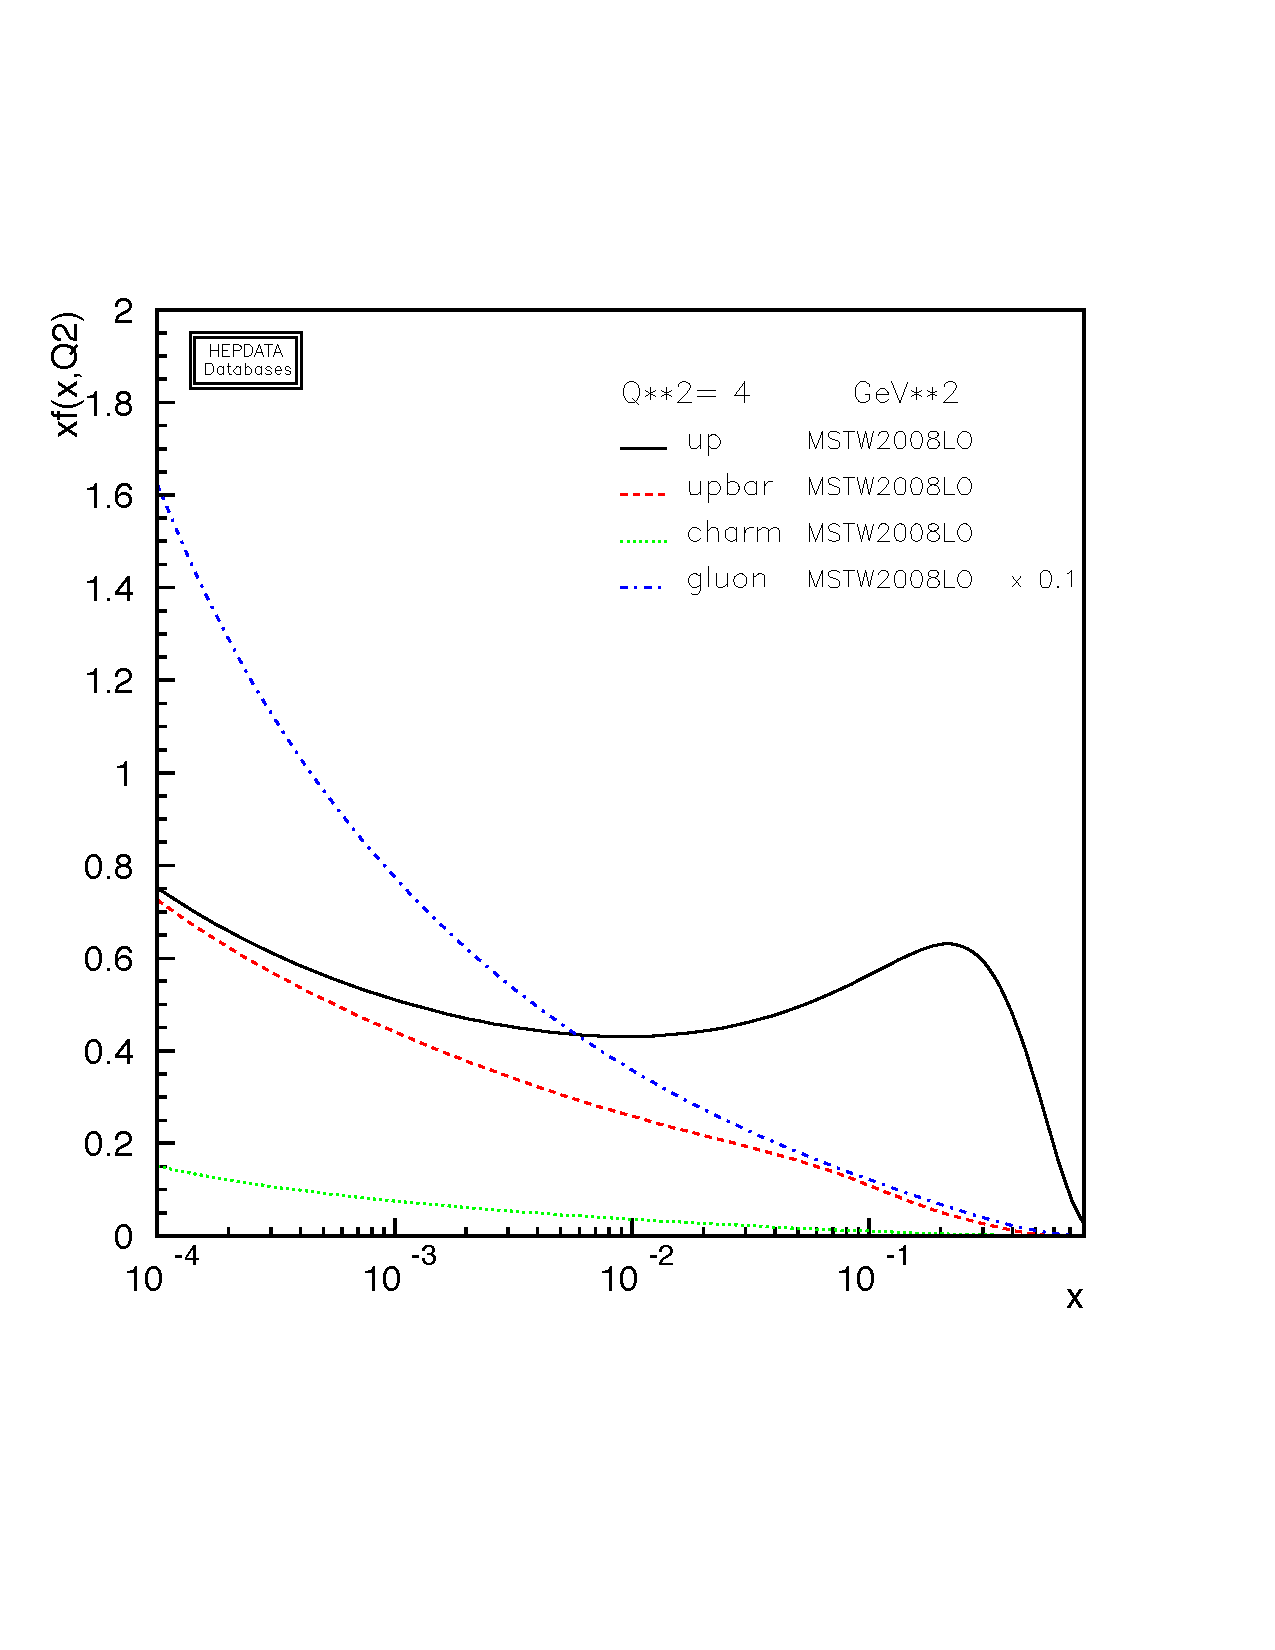
\includegraphics[scale=0.42]{pdfs2gev} \ 
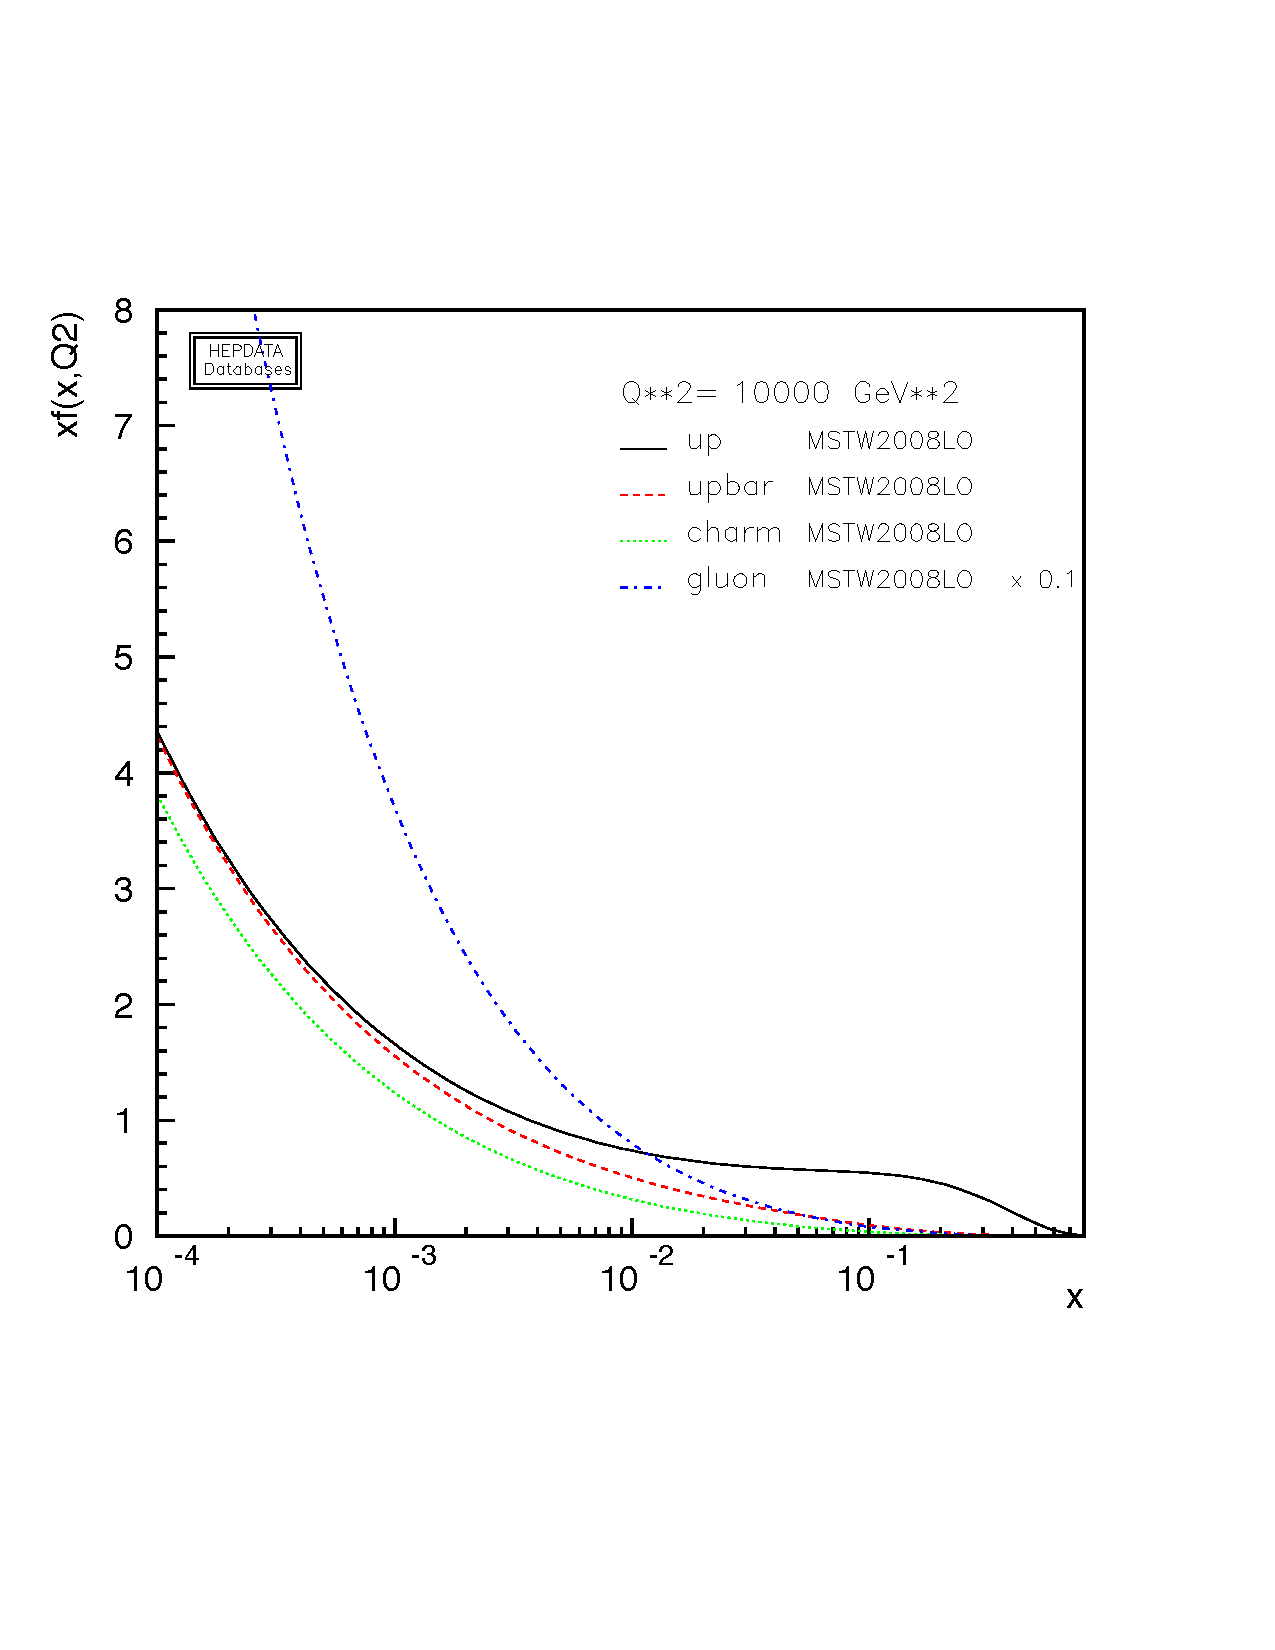
\includegraphics[scale=0.42]{pdfs100gev}
\caption{Illustration of the change of the $u$ (black), $\bar{u}$ (red, dashed),
 $c$ (green, dotted), and $g$ (blue, dot-dashed) distributions, from 
$Q=\mu_F= 2\,\mathrm{GeV}$ (left) to $Q = \mu_F = 100\,\mathrm{GeV}$ (right). 
Note that a factor 0.1 has been
 applied to the gluon distribution. Plots made using the HEPDATA online
 tool~\cite{Buckley:2010jn}.\label{fig:pdfEvol}}
\end{figure}
\index{Quarks!PDFs}%
\index{Gluons!PDFs}%
The behavior 
of the PDFs as we evolve $\mu_F$ from a low scale, 2 GeV, to a high one, 100
GeV, is illustrated in \figRef{fig:pdfEvol}, 
for the MSTW\footnote{MSTW: Martin-Stirling-Thorne-Watt.} 2008
LO\footnote{The ``LO'' means 
that the fit was performed using LO matrix elements in the cross section
formulae.} PDF set~\cite{Martin:2009iq}. At low
$Q=\mu_F = 2\,\mathrm{GeV}$ (left), the proton structure is dominated by a few hard
quarks (a ``valence bump'' is clearly visible around $x \sim 0.2$), 
while at
higher scales $Q = 100\,\mathrm{GeV}$ (right) we predominantly resolve fluctuations
within fluctuations, yielding increasingly large gluon- and sea-quark
distributions with rather small $x$ values, while the valence quarks play
a progressively smaller role.

\index{Uncertainties!PDF sets}%
We note that different collaborations, like CTEQ, MSTW, NNPDF, etc., use  different 
ans\"atze for the form of $f(x,\mu_0^2)$. They may also include
different data in the fits, and/or treat or weight the data
differently. Thus, results from different groups may not always be
mutually compatible. 
\begin{figure}[t]
\centering
\includegraphics*[scale=0.45]{pdfunc.pdf}
\caption{Illustration of the difference between the MSTW 2008 and CTEQ6 LO
 gluon PDFs at $\mu_F = 10\,\mathrm{GeV}$. 
All curves are normalized to the central MSTW 2008
 prediction. The black solid lines show the 90\% CL MSTW variations,
 while the dashed red line shows the CTEQ6L1 distribution.\label{fig:pdfUnc}}
\end{figure}
An example is given in \figRef{fig:pdfUnc}, which shows the difference
 between the CTEQ6L1 gluon PDF~\cite{Pumplin:2002vw}~(red dashed) and
 the MSTW 2008 LO 
 one~\cite{Martin:2009iq}, normalized to MSTW  (which would thus
 be a flat line at zero),  at $\mu_F=10\,\mathrm{GeV}$. 
The $y$ axis shows the relative difference between the sets, in per
 cent. Also shown are 
 the 90\% CL contours computed from the uncertainty variations included in the 
MSTW 2008 LO set (black). Using only the MSTW uncertainty band, 
 one would arrive at an estimated $\sim 5\%$ uncertainty over most of
 the $x$ range, while including the CTEQ6L1 set would increase that to
 $\sim 10\%$. At NLO, this discrepancy is reduced, but not removed.
 A significant effort is currently being undertaken within the PDF community 
to agree on common, and more comprehensive, ways of defining PDF uncertainty
bands~\cite{Alekhin:2011sk,Watt:2012tq}. This is complicated due to the
 different ways of defining $f(x,\mu_0^2)$ and due to 
the experimental data sets not always
being fully compatible with one another. For the
time being, it is recommended to try at least sets from two different
groups, for a comprehensive uncertainty estimate. 

\index{Structure functions}%
Occasionally, the words \emph{structure functions} and \emph{parton
densities} 
are
used interchangeably. However, there is an important distinction between
the two, which we find often in (quantum) physics: the former is a
physical observable used to parametrize the DIS cross sections (see
e.g.~\cite{Dissertori:2003pj}), while the latter is a ``fundamental''
quantity extracted from it. In particular, since the parton densities
are not, themselves, physically observable, they can only be defined
within a specific factorization scheme, order by order in perturbation
theory. The only exception is at leading order, at which they have the
simple physical interpretation of parton number densities. When going to
higher orders, we tend to keep the simple intuitive picture from LO in
mind, but one should be aware that the fundamental relationship between
PDFs and measured quantities is now more complicated (due to the
interplay between the PDFs and the real and virtual corrections to the
LO cross section), and that the parton densities no longer have a clear
probabilistic interpretation starting from NLO. 

\begin{figure}[t]
\centering
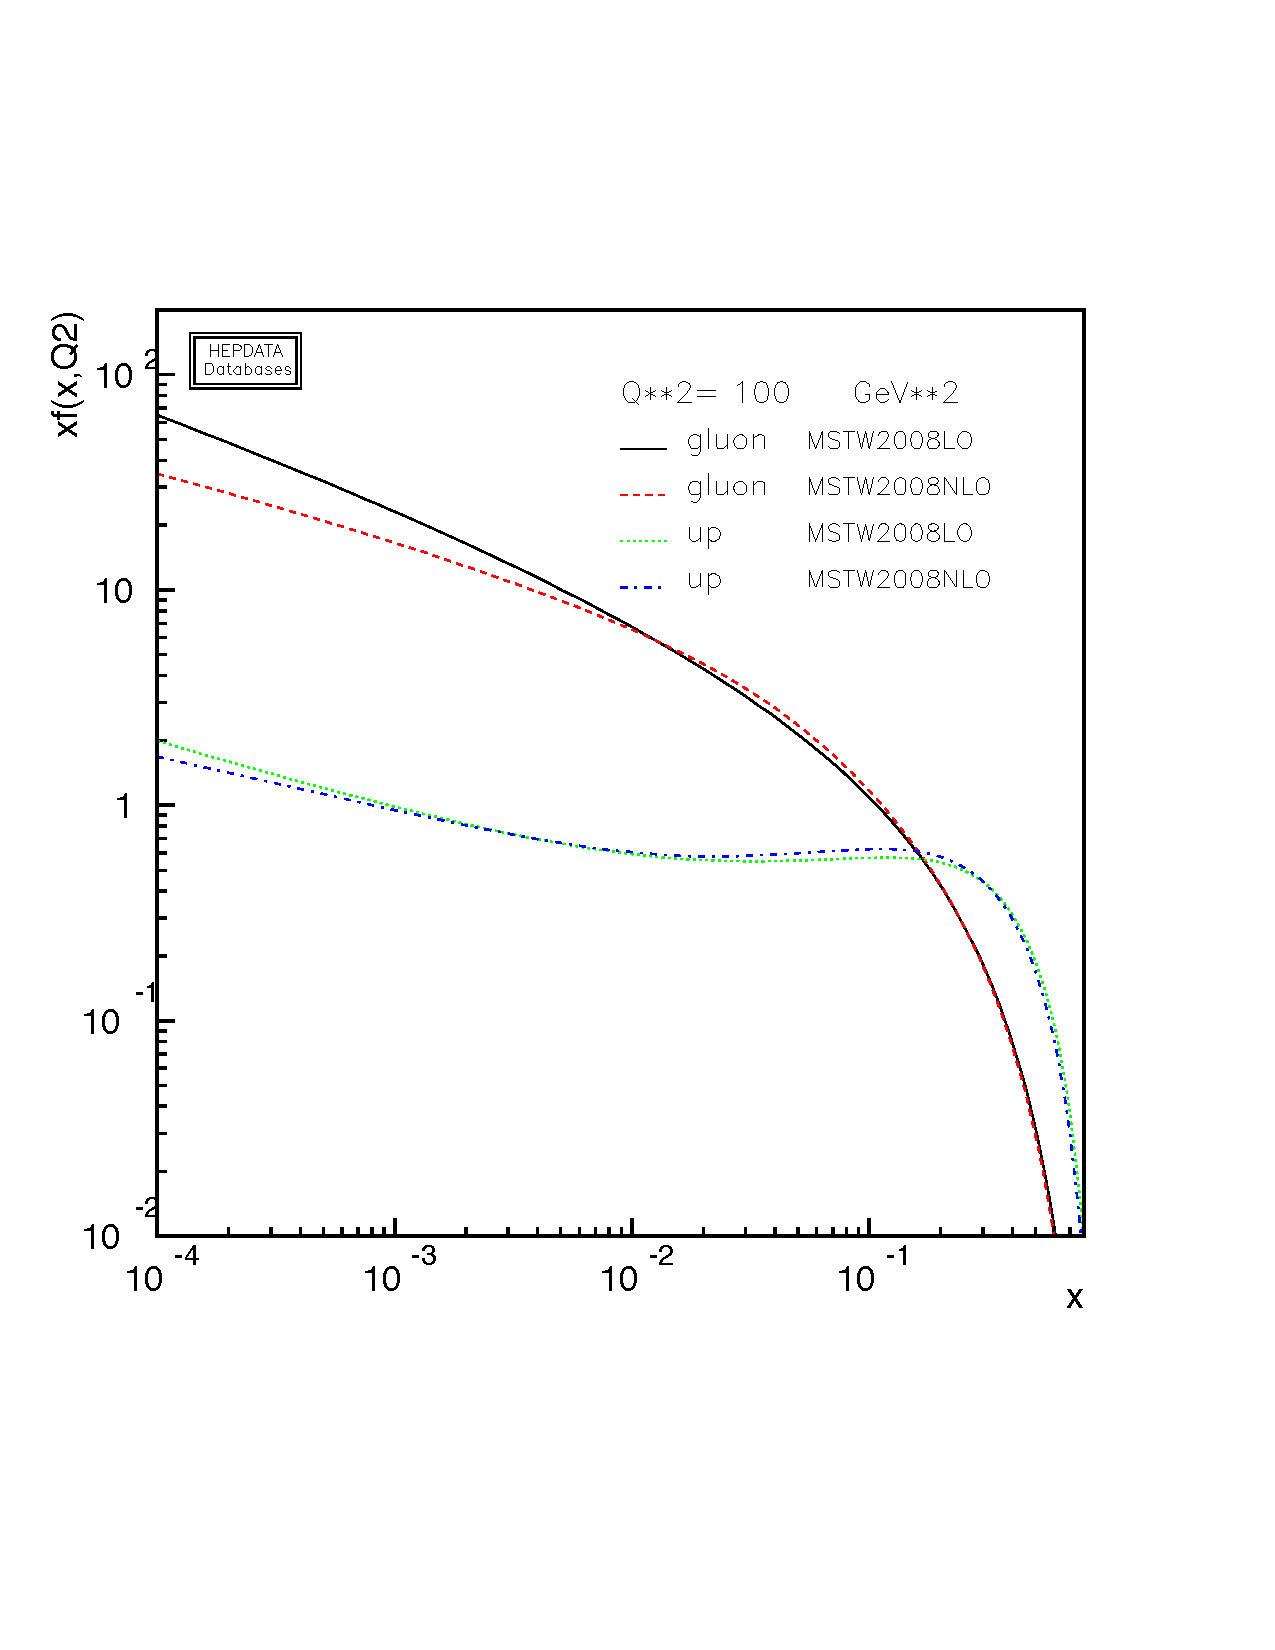
\includegraphics[scale=0.42]{pdforders}
\caption{Illustration of the change between PDF fits using LO and NLO
 matrix elements: the $g$ distribution at LO (black) and NLO (red,
 dashed), and the $u$ distribution at LO (green, dotted) and NLO (blue,
 dot-dashed), for the MSTW 2008 PDF sets~\cite{Martin:2009iq}, 
at $Q = \mu_F = 10\,\mathrm{GeV}$. 
Plots made using the HEPDATA online 
 tool~\cite{Buckley:2010jn}.\label{fig:pdforders}}
\end{figure}
The reader should also be aware that there is some ambiguity whether 
NLO PDFs should be used for 
 LO calculations. In principle, the higher-order PDFs are better
  constrained and the difference between, e.g., an NLO and an LO set
  should formally be beyond LO precision, so that one might be tempted
  to simply use the highest-order available PDFs for any calculation. 
  However, higher-order terms can sometimes be absorbed, at least partially,
  into effective lower-order  coefficients. In the
  context of PDFs, the fit parameters of lower-order PDFs will 
  attempt to compensate for missing higher-order
  contributions in the matrix 
  elements. To the extent those higher-order contributions are
  \emph{universal}, this is both desirable and
  self-consistent. This leads to some typical qualitative differences
  between LO and NLO PDFs, illustrated in \figRef{fig:pdforders}: 
  NLO PDFs tend to be smaller at low $x$ and
      slightly larger at high $x$, than LO ones. Thus, it is quite
      possible that using an NLO PDF in conjunction with LO matrix
      elements can give a worse agreement with data than LO PDFs do. 

\index{Monte Carlo!Event generators}%
\index{Parton showers}%
\index{Parton showers!Initial-state evolution}%
Finally, another oft-raised question concerns which PDF sets to use for the
  parton-shower evolution in Monte Carlo
  generators. Importantly, the equations driving the 
initial-state showers in Monte Carlo models are only sensitive to 
\emph{ratios} of PDFs~\cite{Bengtsson:1986gz}. Since the shower
  evolution typically 
  only has leading-logarithmic (LL) precision, it should be
  theoretically consistent to use any (LO or better) 
PDF set to drive the
  evolution. However, similarly to above, there will be subleading
  differences between different choices, and one is justified in
  worrying about the level of physical effects that could be generated. 
Unfortunately, there is 
  currently no way to ensure 100\% self-consistency. 
  Since PDF fits are not done with MC codes, but
  instead use analytical resummation models (see, e.g., the TASI
  lectures by Sterman~\cite{Sterman:1995fz}), which are not identical to
  their MC counterparts, the PDF fits are essentially ``tuned'' to a
  slightly different resummation than that incorporated in a given MC
  model. In practice, not much is known about the size and impact
  of this ambiguity~\cite{Gieseke:2004tc}. Known differences include: 
  the size of phase space (purely collinear massless PDF evolution
  vs.\ the finite-transverse-momentum massive  MC phase space),  
  the treatment of momentum conservation and recoil effects,
  additional higher-order effects explicitly or implicitly included in
  the MC evolution, choice of renormalization scheme
  and scale, and, for those MC algorithms that do not rely on
  collinear (DGLAP, see \cite{Dissertori:2003pj}) 
  splitting kernels (e.g., the various kinds of dipole
  evolution algorithms, see \cite{Bern:2008ef}), differences in the
  effective factorization 
  scheme. 

As a baseline, we recommend simply using whatever PDF set the given MC
  model was originally tuned with, since this should de facto  (by
  fitting the available 
  data) reabsorb as much of the inconsistency as
  possible. Furthermore, it should be emphasized that underlying-event
  and minimum-bias models 
  based on multi-parton interactions
  (see \secRef{sec:soft-processes}) usually make the explicit
  assumption 
that 
  the PDFs can be interpreted as physical number densities even 
  down to very low $Q$ and $x$, a property which is generally 
  only true for LO PDFs. It must therefore be strongly discouraged to use 
  (N)NLO PDF sets in this context. 

\subsection{Fixed-Order QCD \label{sec:fixed-order}}
\index{Matrix elements}%

Consider the production of an arbitrary final state, $F$ (e.g., a
Higgs boson, a $t\bar{t}$ pair, etc). 
Schematically, we may  express the (perturbative) all-orders
differential cross section for an observable \obs, 
in the following way:
\begin{equation}
\left.\frac{\dd{\sigma_F}}{\dd{\obs}}\right\vert_{\textcolor{blue}{\mrm{ME}}}
= \underbrace{\sum_{k=0}^\infty\int \dPS{F+k} }_{\Sigma~\mbox{legs}} 
 \Big\vert \underbrace{\sum_{\ell=0}^{\infty} {\cal
   M}_{F+k}^{(\ell)}}_{\Sigma~\mbox{loops}} \Big\vert^2 \,
\delta\left(\obs-\obs(\PS{F+k})\right)~,\label{eq:fixed-order}
\end{equation}
where, for compactness, we have suppressed all PDF and luminosity
normalization factors. 
${\cal M}_{F+k}^{(\ell)}$ is the amplitude for producing $F$ in
association with $k$ additional final-state partons, ``legs'', 
and with $\ell$ additional loops. The sums start at $k=0$ and $\ell=0$,
corresponding to the Leading Order for producing $F$, while higher terms
represent real and virtual corrections, respectively. 

The purpose of the $\delta$ function is
to project out hypersurfaces of constant value of \obs\ 
in the full $\dPS{F+k}$ phase space, with $\obs(\PS{F+k})$ a function that
defines $\obs$ evaluated on each specific momentum configuration, 
$\PS{F+k}$. (Without the 
$\delta$ function, the formula would give the total integrated
cross section, instead of the cross section differentially in $\obs$.) 

We recover the various fixed-order truncations of perturbative QCD
\index{pQCD} (pQCD) 
by limiting the
nested sums in \eqRef{eq:fixed-order} to include only specific values
of $k+\ell$. Thus, 
\index{LO}%
\index{NLO}%
\index{NNLO}%
\index{Jets}
\begin{center}
\begin{tabular}{lcp{9.5cm}}
$k=0$, $\ell=0$ &$\implies$& Leading Order  (usually tree-level) 
for $F$ production\\[2mm]
$k=n$, $\ell=0$ &$\implies$& Leading Order for $F+n\,$jets\\[2mm]
$k+\ell\le n$,  &$\implies$& N$^n$LO for $F$ {\small (includes N$^{n-1}$LO for
  $F+1\,$jet, N$^{n-2}$LO for $F+2\,$jets, and so on up to LO for $F+n\,$jets)}~.\\
\end{tabular}
\end{center}

\index{Collinear limit}%
\index{Soft limit}%
For $k\ge1$, we are  not considering inclusive
$F$ production; instead, we are considering the process
$F+k$ jets. If we simply  
integrate over all momenta, as implied by the integration over \dPS{F+k}
in \eqRef{eq:fixed-order}, we would be including configurations in
which one or more of the $k$ partons are collinear or soft. Such
configurations are infrared divergent in QCD and hence must be
\index{Infrared divergences}
regulated. Since we talk about \emph{collinear} and \emph{soft}
divergences (the origins of which will be discussed in more detail
in \secsRef{sec:subtraction} and \ref{sec:parton-showers}), 
cuts on \emph{angles} and \emph{energies} and/or cuts on
combinations, like \emph{transverse momenta}, can be used
to cut away the problematic regions of phase space. 

Recall, however, that pQCD is approximately scale invariant. This
implies that 
\index{QCD!Scale invariance}%
a regularization cut on a dimensionful quantity, like energy or
transverse momentum, should be formulated as a \emph{ratio} of scales,
rather than as an absolute number. 
\index{LO}%
For example, a jet with $p_\perp = 50\,\mathrm{GeV}$ 
would be considered hard and well-separated if produced in association with
an ordinary $Z$ boson (with hard scale $M_Z=91.2\,\mathrm{GeV}$), 
while the same jet would be considered soft if produced
in association with a 900-GeV $Z'$ boson
(see \cite{Plehn:2005cq,Alwall:2008qv} for more explicit
examples).

\index{NLO!Infrared divergences}%
\index{Infrared divergences}%
The essence of the point is that, 
if the regularization scale is taken too low, logarithmic
enhancements of the type 
\begin{equation}
\alpha_s^n\ln^{m\le 2n}\left(\frac{Q_F^2}{Q_k^2}\right)
\label{eq:logs}
\end{equation}
will generate progressively larger corrections, order by order, which
will spoil any fixed-order truncation of the perturbative
series. Here, $Q_F$ is the hard scale associated with the process
under consideration, while $Q_k$ is the scale associated with an
additional parton, $k$. 

\index{LO}%
A good rule of thumb
is that if $\sigma_{k+1} \approx \sigma_{k}$ (at whatever order you
are calculating), then the perturbative series is 
converging too slowly for a fixed-order truncation
of it to be reliable. For fixed-order perturbation theory to be
applicable, you must place your cuts on the hard process such that 
$\sigma_{k+1} \ll \sigma_{k}$. In the
discussion of parton showers in
\SecRef{sec:parton-showers}, we shall see how the region of
applicability of perturbation theory can be extended.  

\index{NLO}%
\index{Unitarity}%
\index{KLN theorem}%
\index{NLO!Infrared divergences}%
\index{Infrared divergences}%
The virtual amplitudes, for $\ell \ge 1$, are divergent
for any point in phase space. However, as encapsulated by the famous KLN theorem
\cite{Kinoshita:1962ur,Lee:1964is}, unitarity (which essentially
expresses probability conservation) puts a powerful
constraint on the IR divergences\footnote{The loop integrals also
  exhibit UV divergences, but these are dealt with by
  renormalization.}, 
forcing them to cancel exactly 
against those coming from the unresolved real emissions 
that we had to cut out above, order by order, 
making the complete answer for fixed
$k+\ell = n$ finite\footnote{Formally, the KLN theorem states that the
sum over degenerate quantum states is finite. In context of
fixed-order perturbation theory, this is exemplified by states with infinitely
collinear and/or soft radiation being degenerate with the
corresponding states with loop corrections; they cannot be told apart
by any physical observable.}
Nonetheless, since this cancellation happens
between contributions that formally live in different phase spaces, 
a main aspect of loop-level higher-order calculations is how to
arrange for this cancellation in practice, either analytically or 
numerically, with many different methods currently on the market. We
shall discuss the idea behind subtraction approaches 
in \secRef{sec:subtraction}. 

\index{Matrix elements}
A convenient way of illustrating the terms of the perturbative series that
a given matrix-element-based calculation includes is given in
\figRef{fig:loopsnlegs}. 
\begin{figure}[t]\vspace*{-0.15cm}
\begin{center}
\scalebox{0.90}{
\begin{tabular}{l}
\large\bf F @ LO\\[2mm]
\begin{loopsnlegs}[c]{p{0.25cm}|ccccc}
 \small 2&~\wbox{\pqcd[2]{0}} & \wbox{\pqcd[2]{1}} & \ldots \\[2mm]
 \small 1&~\wbox{\pqcd[1]{0}} & \wbox{\pqcd[1]{1}}  
   & \wbox{\pqcd[1]{2}} & \ldots \\[2mm]
 \small 0&~\gbox{\pqcd[0]{0}} & \wbox{\pqcd[0]{1}} 
   & \wbox{\pqcd[0]{2}} 
   & \wbox{\pqcd[0]{3}} & \ldots \\
\hline
& \small 0 & \small 1 & \small 2 & \small 3 & \ldots
 \end{loopsnlegs}\end{tabular}\hspace*{-0.7cm}
\raisebox{0.9cm}{\begin{minipage}{1.9cm}
\center\includegraphics*[scale=0.23]{born.png}
\tiny Max Born, 1882-1970\\
\index{Nobel prize}Nobel 1954
\end{minipage}}%
\begin{tabular}{l}
\large\bf F + 2 @ LO\\[2mm]
\begin{loopsnlegs}[c]{p{0.25cm}|ccccc}
 \small 2&~\wbox{\pqcd[2]{0}} & \wbox{\pqcd[2]{1}} & \ldots
&  \multicolumn{2}{l}{\tiny 
\colorbox{red}{\parbox[b]{1.75cm}{\raggedright\textcolor{white}{LO for $F+2$\\
      $\to \infty$ for $F+1$\\
      $\to \infty$ for $F+0$\\
}}
}} \\[2mm]
 \small 1&~\wbox{\pqcd[1]{0}} & \wbox{\pqcd[1]{1}}  
   & \wbox{\pqcd[1]{2}} & \ldots \\[2mm]
 \small 0&~\wbox{\pqcd[0]{0}} & \wbox{\pqcd[0]{1}} 
   & \gwbox{\pqcd[0]{2}} 
   & \wbox{\pqcd[0]{3}} & \ldots \\
\hline
& \small 0 & \small 1 & \small 2 & \small 3 & \ldots
 \end{loopsnlegs}
\end{tabular}}
\caption{Coefficients of the perturbative series covered by LO calculations. 
{\sl Left:} $F$ production at lowest order. {\sl Right:} $F+2\,$jets at LO, with the
  half-shaded box illustrating the restriction to the region of phase
  space with exactly 2 resolved jets.
  The total power of $\alpha_s$ for each coefficient is $n = k+\ell$. 
(Photo of Max Born from \url{nobelprize.org}).
\label{fig:loopsnlegs}}
\end{center}
\end{figure}
In the left-hand pane, the shaded box corresponds to 
the lowest-order ``Born-level'' matrix element squared. This coefficient 
is non-singular and hence can be integrated over all of phase space,
which we illustrate by letting the shaded area fill all of the
relevant box. 
A different kind of leading-order calculation is illustrated in
the right-hand pane of \figRef{fig:loopsnlegs}, where the shaded box
corresponds to the lowest-order matrix element squared for
$F+2\,$jets. 
\index{Soft limit}\index{Collinear limit}
This coefficient diverges in the part of phase space
where one or both of the jets are unresolved (i.e., soft or collinear), 
  and hence integrations can only cover the hard part of
  phase space, which we reflect by only shading the upper half of
  the relevant box. 

\index{NLO}
\FigRef{fig:loopsnlegs2} illustrates the inclusion of NLO
virtual corrections. 
\begin{figure}[t]
\begin{center}%
\scalebox{0.90}{
\begin{tabular}{l}
\large\bf F @ NLO\\[2mm]
\begin{loopsnlegs}[c]{p{0.25cm}|ccccc}
 \small 2&~\wbox{\pqcd[2]{0}} & \wbox{\pqcd[2]{1}} & \ldots &
 \multicolumn{2}{l}{\tiny 
\colorbox{red}{\parbox[b]{1.75cm}{\raggedright\textcolor{white}{NLO for
      $F+0$\\
$\to$ LO
      for $F+1$}}
}}
\\[2mm]
 \small 1&~\gbox{\pqcd[1]{0}} & \wbox{\pqcd[1]{1}}  
   & \wbox{\pqcd[1]{2}} & \ldots \\[2mm]
 \small 0&~\gbox{\pqcd[0]{0}} & \gbox{\pqcd[0]{1}} 
   & \wbox{\pqcd[0]{2}} &\wbox{\pqcd[0]{3}} & \ldots \\
\hline
& \small 0 & \small 1 & \small 2 & \small 3 & \ldots
 \end{loopsnlegs}
\end{tabular}\hspace*{-1mm}
\begin{tabular}{l}
\large\bf F+1 @ NLO\\[2mm]
\begin{loopsnlegs}[c]{p{0.25cm}|ccccc}
 \small 2&~\wbox{\pqcd[2]{0}} & \wbox{\pqcd[2]{1}} & \ldots &
 \multicolumn{2}{l}{\tiny 
\colorbox{red}{\parbox[b]{1.75cm}{\raggedright\textcolor{white}{NLO for
      $F+1$\\
     $\to$ LO
      for $F+2$ \\$\to \infty$ for $F + 0$}}
}}
\\[2mm]
 \small 1&~\wbox{\pqcd[1]{0}} & \gwbox{\pqcd[1]{1}}  
   & \wbox{\pqcd[1]{2}} & \ldots \\[2mm]
 \small 0&~\wbox{\pqcd[0]{0}} & \gwbox{\pqcd[0]{1}} 
   & \gwbox{\pqcd[0]{2}} 
   & \wbox{\pqcd[0]{3}} & \ldots \\
\hline
& \small 0 & \small 1 & \small 2 & \small 3 & \ldots
 \end{loopsnlegs}
\end{tabular}}
\caption{Coefficients of the perturbative series covered by NLO calculations. 
{\sl Left:} 
   $F$ production at NLO. {\sl Right:} $F+1\,$jet at NLO, with
  half-shaded boxes illustrating the restriction to the region of phase
  space with exactly 1 resolved jet.
  The total power of $\alpha_s$ for each coefficient is $n = k+\ell$.
\label{fig:loopsnlegs2}}
\end{center}
\end{figure}
To prevent confusion, first a point on notation: by 
$\sigma_0^{(1)}$, we intend
\begin{equation}
\sigma_0^{(1)} = \int \dPS{0} \, 2\mrm{Re}[{\cal M}_{0}^{(1)} {\cal M}_0^{(0)*}]~,
\end{equation}
which is of order $\alpha_s$ relative to the Born
level. 
\index{NLO}
\index{NNLO}
Compare, e.g., with the expansion of
\eqRef{eq:fixed-order} to order $k+\ell = 1$. In particular, $\sigma_0^{(1)}$
should \emph{not} be confused with the integral over the 1-loop matrix
element squared (which would be of relative order $\alpha_s^2$ and
hence forms part of the NNLO coefficient $\sigma_0^{(2)}$). Returning
to \figRef{fig:loopsnlegs2}, the unitary cancellations between real
and virtual singularities imply that we can now extend the
integration of the real correction in the left-hand pane over all of
phase space, while retaining a finite total cross section,
\index{NLO}
\begin{equation}
\begin{array}{rclll}
\displaystyle\sigma^\mrm{NLO}_0 & = 
 &\displaystyle\int \dPS{0} |{\cal M}^{(0)}_0|^2 
 & \displaystyle + \int \dPS{1}|{\cal M}^{(0)}_1|^2
 & \displaystyle + \int \dPS{0} \,2\mrm{Re}[{\cal M}_{0}^{(1)} {\cal M}_0^{(0)*}] 
\\[6mm]
 & = &\displaystyle \sigma^{(0)}_0
 & \displaystyle +\ \sigma^{(0)}_{1}
 & \displaystyle +\ \sigma^{(1)}_{0} 
~,\end{array} \label{eq:sigmaNLO}
\end{equation}
with $\sigma_0^{(0)}$ the finite Born-level cross section, 
and the positive divergence caused by integrating the second term over
all of phase space  is canceled by a negative one coming from the
integration over loop momenta in 
the third term. One method
for arranging the cancellation of singularities  --- subtraction --- is 
discussed in \secRef{sec:subtraction}. 

However,  if our starting point for the NLO
calculation is a process which already has a non-zero number of hard
jets, we must 
continue to impose that at least that number of jets must still be resolved in the
final-state integrations,
\begin{equation}
\begin{array}{rclll}
\displaystyle\sigma^\mrm{NLO}_1(\ptmin) & = 
 & \displaystyle
   \int_{\pt>\ptmin}\hspace*{-11mm} \dPS{1}\, |{\cal M}^{(0)}_1|^2
 & \displaystyle 
   + \int_{\pt[1]>\ptmin}\hspace*{-11mm} \dPS{2}\,
   |{\cal M}^{(0)}_2|^2
 &\displaystyle 
   + \int_{\pt>\ptmin}\hspace*{-11mm} \dPS{1} \, 
   2\mrm{Re}[{\cal M}_{1}^{(1)} {\cal M}_1^{(0)*}] 
\\[6mm]
 & = &\displaystyle \sigma^{(0)}_1(\pt>\ptmin)
 & \displaystyle +\ \sigma^{(0)}_{2}(\pt[1]>\ptmin)
 & \displaystyle +\ \sigma^{(1)}_{1}(\pt>\ptmin)
~,\end{array}\label{eq:sigmanlo1}
\end{equation}
where the restriction to at least one jet having 
$\pt>\ptmin$ has been illustrated in the right-hand 
pane of \figRef{fig:loopsnlegs2} by shading only the upper part of the
relevant boxes. In the second term in \eqRef{eq:sigmanlo1}, 
the notation $\pt[1]$ is used to
\index{Jets}
denote that the integral runs over the phase space in which at least
one ``jet'' (which may consist of one or two partons) must be resolved
with respect to $\ptmin$. Here, therefore, an explicit dependence on
the algorithm used to define ``a jet'' enters for the first time. This
is discussed in more detail in the 2009 ESHEP lectures by Salam
\cite{Salam:2010zt}. 
\index{Jets}%
\index{Jets!Definitions|see{\cite{Salam:2010zt}}}
\index{Jets!Algorithms|see{\cite{Salam:2010zt}}}

\index{NNLO}%
To extend the integration to cover also the case of 2 unresolved jets,
we must combine the left- and right-hand parts of
\figRef{fig:loopsnlegs2} and add the new coefficient
\begin{equation}
\sigma_0^{(2)} = |{\cal M}_0^{(1)}|^2 + 2\mrm{Re}[ {\cal
    M}_0^{(2)}{\cal M}_0^{(0)*} ]~,
\end{equation}
 as illustrated by the diagram in \figRef{fig:loopsnlegs3}. 
\begin{figure}[t]
\scalebox{0.90}{\large\bf F @ NNLO}
\begin{center}
\scalebox{0.90}{
\begin{loopsnlegs}[c]{p{0.25cm}|ccccc}
 \small 2&~\gbox{\pqcd[2]{0}} & \wbox{\pqcd[2]{1}} & \ldots &
 \multicolumn{2}{l}{\tiny 
\colorbox{red}{\parbox[b]{1.75cm}{\raggedright\textcolor{white}{NNLO for
      $F+0$\\
     $\to$ NLO
      for $F+1$ \\$\to$ LO for $F + 2$}}
}}
\\[2mm]
 \small 1&~\gbox{\pqcd[1]{0}} & \gbox{\pqcd[1]{1}}  
   & \wbox{\pqcd[1]{2}} & \ldots \\[2mm]
 \small 0&~\gbox{\pqcd[0]{0}} & \gbox{\pqcd[0]{1}} 
   & \gbox{\pqcd[0]{2}} &\wbox{\pqcd[0]{3}} & \ldots \\
\hline
& \small 0 & \small 1 & \small 2 & \small 3 & \ldots
 \end{loopsnlegs}}
\caption{Coefficients of the perturbative series covered by an NNLO
  calculation. 
  The total power of $\alpha_s$ for each coefficient is $n =
  k+\ell$. Green  shading represents the full perturbative 
  coefficient at the respective $k$ and $\ell$.
\label{fig:loopsnlegs3}}
\end{center}
\end{figure}

\index{NLO}
\index{Subtraction}
\index{Unitarity}
\index{KLN theorem}
\subsection{The Subtraction Idea \label{sec:subtraction}}
According to the KLN theorem, the IR singularities coming from
integrating over collinear and soft real-emission configurations
should cancel, order by order, by those coming from the IR divergent
loop integrals. This implies that we should be able to rewrite e.g.\
the NLO cross section, \eqRef{eq:sigmaNLO}, as 
\begin{eqnarray}
\displaystyle\sigma^\mrm{NLO} 
 & = &\displaystyle \sigma^\mathrm{Born}
\ + \ \mathrm{Finite}\left\{\int \dPS{F+1} |{\cal M}^{(0)}_{F+1}|^2\right\}
\ + \ 
\mathrm{Finite}\left\{\int \dPS{F} \, 2\mrm{Re}[{\cal M}_{F}^{(1)} {\cal M}_{F}^{(0)*}]\right\} 
\displaystyle ~,
\end{eqnarray}
with the second and third terms having had their common (but
opposite-sign) singularities canceled out and some explicitly finite
quantities remaining. 

The first step towards this goal is to classify all IR singularities
that could appear in the amplitudes. We know that the IR limits are
universal, so they can be classified using a set of
process-independent functions that only has to be worked out once and
for all. A widely used such set of functions are the 
\index{Catani-Seymour dipoles}
\emph{Catani-Seymour} (CS) dipole ones~\cite{Catani:1996vz,Catani:1996jh},
a method which by now has even been partially automated~\cite{Nagy:2003tz,Frederix:2008hu}. 
Here,  
\index{Antennae}
we shall instead use a formalism based
on \emph{antennae}~\cite{Kosower:1997zr,Kosower:2003bh,GehrmannDeRidder:2005cm}.    
\index{NLO}The distinction between the two is basically that one antenna is made
up of two dipole ``ends'', hence the antenna formalism tends to
generate somewhat fewer terms. At NLO, however, there is no fundamental
incompatibility --- the antennae we use here can always be
partitioned into two dipole ends, if so desired. (Note: 
\index{NNLO}%
\index{Sector decomposition}%
only the antenna method has been 
successfully generalized to 
NNLO~\cite{GehrmannDeRidder:2007hr,Weinzierl:2008iv}. Other NNLO 
techniques, not covered here, are \emph{sector decomposition}, 
see \cite{Heinrich:2008si,Boughezal:2011jf}, and the generic formalism 
for hadroproduction of colorless states presented in~\cite{Catani:2007vq}.)

\index{NLO}
\index{Subtraction}
At NLO, the idea with subtraction is thus to rewrite the NLO cross section
by adding and subtracting a simple function, $\dd{\sigma_S}$, 
that encapsulates all the
IR limits, 
\index{Kinoshita-Lee-Nauenberg|see{KLN theorem}}
\index{KLN theorem}
\begin{eqnarray}
\sigma^\mrm{NLO} & = & 
 \sigma^\mathrm{Born} 
 \ + \ \int \dPS{F+1} \underbrace{\left(|{\cal M}^{(0)}_{F+1}|^2
{\color{red}{ \ - \ \dd{\sigma_S^\mrm{NLO}}}}\right)}_{\mbox{Finite by
Universality}} \nonumber \\[2mm]
&& \ + \ \underbrace{\int \dPS{F} \, 2\mrm{Re}[{\cal M}_{F}^{(1)} {\cal
M}_F^{(0)*}] \ {\color{red}+} \int \dPS{F+1} {\color{red}\dd{\sigma_S^\mrm{NLO}}}
}_{\mbox{Finite by KLN}}~.\label{eq:subtraction}
\end{eqnarray}
The task now is to construct a suitable form for $\dd{\sigma_S}$. A
main requirement is that it 
should be sufficiently simple that the integral in the last term can
be done analytically, in dimensional regularization, 
so that the IR poles it generates can be canceled against those
from the loop term.

\index{Soft limit}
\index{Eikonal}
To build a set of universal terms that parametrize the IR singularities of
any amplitude, we start from the observation that gauge theory
amplitudes factorize in the \emph{soft limit}, as follows:
\begin{eqnarray}
\left\vert{\cal M}_{F+1} (\ldots, i,j,k, \ldots )\right\vert^2
  & \stackrel{j_g\to 0}{\to} & g_s^2\ N_C \left( \frac{2 s_{ik}}{s_{ij}
  s_{jk}} - \frac{2m_i^2}{s_{ij}^2} - \frac{2 m_k^2}{s_{jk}^2}\right) 
\left\vert{\cal M}_{F} (\ldots, i,k, \ldots )\right\vert^2
~,\label{eq:eikonal}
\end{eqnarray}
\index{Color connections}%
where parton $j$ is a soft gluon, partons 
$i$, $j$, and $k$ form a chain of color-space index contractions 
(we say they are \emph{color-connected}), 
$g_s$ is the strong coupling, 
and the terms in parenthesis are 
\index{Eikonal}%
\index{Soft eikonal|see{Eikonal}}%
\index{Color factors}%
called the \emph{soft eikonal factor}. We here show it including 
mass corrections, which appear if $i$ and $k$ have non-zero rest
masses, with the invariants 
$s_{ab}$ then defined as 
\begin{equation}
s_{ab} \equiv 2p_a\cdot p_b = (p_a+p_b)^2 - m_a^2 - m_b^2~.
\end{equation}
The color factor, $N_C$, is valid for the leading-color
contribution, regardless of whether the $i$ and $k$ partons are quarks
or gluons. At subleading color, an additional soft-eikonal
factor identical to the one above but with a color factor 
proportional to $-1/N_C$ arises for each $q\bar{q}$ pair
combination. 
\index{CA@$C_A$}
\index{CF@$C_F$}
This, e.g., modifies the effective color factor for $q\bar{q}\to
qg\bar{q}$ from $N_C$ to $N_C(1-1/N_C) = 2C_F$, in agreement with the
color factor for quarks being $C_F$ rather than $C_A$.

\index{Collinear limit}%
\index{DGLAP kernels}%
Similarly, amplitudes also factorize in the \emph{collinear limit}
(partons $i$ and $j$ parallel, so $s_{ij}\to 0$), in which
the eikonal factor above is replaced by the 
famous Dokshitzer-Gribov-Lipatov-Altarelli-Parisi (DGLAP)
splitting kernels~\cite{Gribov:1972ri,Altarelli:1977zs,Dokshitzer:1977sg}, 
which 
were already mentioned in \secRef{sec:pdfs}, in 
the context of PDF evolution. 
They are also the basis of conventional 
parton-shower models, to which we return in \secRef{sec:parton-showers}. 

Essentially,
what antenna functions, CS dipoles, and the like, all do, is to 
combine the soft (eikonal) and
collinear (Altarelli-Parisi) limits into one universal set of functions
that achieve the correct limiting behavior for \emph{both} 
\index{Antennae}
soft and collinear radiation. 
To give an explicit example, the \emph{antenna function} for gluon
emission from a color-connected $q\bar{q}$ pair can be derived from
the matrix elements squared for the process $Z^0 \to q\bar{q} \to
qg\bar{q}$~\cite{Gustafson:1987rq}, 
\index{Eikonal}
\begin{equation}
\frac{\left\vert{\cal M}(Z^0\to q_i g_j \bar{q}_k)\right\vert^2}
{\left\vert{\cal M}(Z^0\to q_I \bar{q}_K)\right\vert^2}
\ = \ g_s^2 \,
2C_F \, \left[ \underbrace{\frac{2s_{ik}}{s_{ij}s_{jk}}}_{\mrm{eikonal}}
+ \frac{1}{s_{IK}}\underbrace{\left(
\frac{s_{jk}}{s_{ij}}
+ \frac{s_{ij}}{s_{jk}}
\right)}_\mrm{collinear} \right]~,\label{eq:subZ}
\end{equation}
where we have neglected mass corrections
(see~\cite{GehrmannDeRidder:2009fz,GehrmannDeRidder:2011dm} for
massive expressions) 
and we recognize the universal eikonal soft factor from \eqRef{eq:eikonal}
in the first term. The two additional terms are less singular, and are
required to obtain the correct collinear (Altarelli-Parisi) 
limits as $s_{ij}\to 0$ or $s_{jk} \to 0$. 

However, since the singularity structure is universal, we could
equally well have used the process
$H^0 \to q\bar{q} \to qg\bar{q}$ to derive the antenna function.
Our antenna function would then have come out as~\cite{GehrmannDeRidder:2011dm},
\index{Eikonal}
\begin{equation}
\frac{\left\vert{\cal M}(H^0\to q_i g_j \bar{q}_k)\right\vert^2}
{\left\vert{\cal M}(H^0\to q_I \bar{q}_K)\right\vert^2}
\ = \ g_s^2 \,
2C_F \, \left[ \underbrace{\frac{2s_{ik}}{s_{ij}s_{jk}}}_{\mrm{eikonal}}
+ \frac{1}{s_{IK}}\underbrace{\left(
\frac{s_{jk}}{s_{ij}}
+ \frac{s_{ij}}{s_{jk}}
\right)}_\mrm{collinear}
+ \underbrace{\frac{2}{s_{IK}}}_{\mrm{finite}}\right]~,
\label{eq:subH}
\end{equation}
where the additional term $2/s_{IK}$ is non-singular (``finite'') over
all of phase space. Thus, we here see an explicit example that the
singularities are process-independent 
while the non-singular terms are process-dependent. 
Since we add and subtract
the same term in \eqRef{eq:subtraction}, the final answer does not depend
on the choice of finite terms. 
\index{Subtraction schemes}
\index{Antennae}
\index{Antenna functions|see{Antennae}}
We say that they correspond to different \emph{subtraction
schemes}. One standard antenna subtraction scheme, which uses the
antenna function defined in \eqRef{eq:subZ} rather than the one
in \eqRef{eq:subH}, is the Gehrmann-Gehrmann-de Ridder-Glover (GGG)
one, given in \cite{GehrmannDeRidder:2005cm}. 

If there is more than one color antenna in the Born-level process, the
form of $\dd{\sigma_S}$ is obtained as a sum over terms, each of which
captures one specific soft limit and either all or ``half'' of a
collinear one, depending on the specific scheme and the type of
parton,
\index{Subtraction}
\begin{equation}
\dd{\sigma_S} \ = \ \sum_{j} A_{IK\to ijk} \, 
\left\vert {\cal M}_F(\ldots,I,K,\ldots)\right\vert^2~,
\end{equation}
with the sum running over all  singular 
$3\to 2$ ``clusterings'' of the $(F+1)$-parton state to $F$
partons. An analysis of the different ways of partitioning the collinear
singularity of gluons among neighboring antenna is beyond the scope of
this introduction, but useful discussions can be found
in~\cite{Larkoski:2009ah,Giele:2011cb,LopezVillarejo:2011ap}. 

\index{Jets!Infrared safety}%
\index{Infrared safety}%
\index{pQCD}%
\subsection{Infrared Safety \label{sec:IRsafe}}
A further requirement for being able to perform calculations within
perturbative QCD is that the observable be \emph{infrared safe}. 
Note: by ``infrared'',
we here mean any  limit 
that involves a low scale (i.e., any non-UV limit), 
without regard to  whether it is collinear or soft.

The property of infrared safety defines a special class of observables which
have \emph{minimal sensitivity} 
to long-distance physics, and which can be consistently computed in
pQCD. 
An observable is infrared safe if:
\begin{enumerate}
\item \index{Soft limit}{\sl(Safety against soft radiation):} Adding any number of infinitely soft particles should not change
  the value of the observable. 
\item \index{Collinear limit}{\sl(Safety against collinear radiation):} Splitting an existing particle up into two comoving particles, with
arbitrary fractions $z$ and $1-z$, respectively, of 
the original momentum, should not change the value of the
observable. 
\end{enumerate}
If both of these conditions are satisfied, any long-distance non-perturbative
corrections will be suppressed by the ratio of the 
long-distance scale to the short-distance one to some
(observable-dependent) power, typically
\index{Infrared safety}%
\index{Jets!Infrared safety}
\begin{equation}
\mbox{IR Safe Observables: IR corrections~~~$\propto$~~~} \frac{Q_{\mathrm{IR}}^2}{Q_{\mathrm{UV}}^2} 
\end{equation}
where $Q_\mathrm{UV}$ denotes
a generic hard scale in the problem, and $Q_\mrm{IR} \sim
\Lambda_\mrm{QCD} \sim \mathcal{O}(\mrm{1\ GeV})$. 

Due to this \emph{power suppression}, 
IR safe observables are not so sensitive to our lack
of ability to solve the strongly coupled IR physics, unless of course
we go to processes for which the relevant hard scale, $Q_{\mrm{UV}}$, is small
(such as minimum-bias, soft jets, or small-scale jet substructure). 
Even when a high scale is present, however, as in resonance decays, jet
fragmentation, or underlying-event-type studies, infrared safety only
guarantees us that infrared corrections are small, not that they are zero. 
Thus, ultimately, we run into a precision barrier even for IR safe observables, 
which only a reliable understanding of the
long-distance physics itself can address. 

To constrain models of long-distance physics, one needs 
infrared \emph{sensitive} observables.
Hence it is not always the case that infrared safe
observables are preferable --- the purpose decides the tool.
Instead of the suppressed corrections above, the perturbative
prediction for such observables contains logarithms of the type
already encountered in \eqRef{eq:logs},
\index{Infrared safety}%
\index{Jets!Infrared safety}%
\begin{equation}
\mbox{IR Sensitive Observables: IR Corrections~~~$\propto$~~~} 
\alpha_s^n\log^{m\le
2n}\left(\frac{Q_{\mathrm{UV}}^2}{Q_{\mathrm{IR}}^2}\right)~,
\end{equation}
 which grow
increasingly large as $Q_{\mathrm{IR}}/Q_{\mathrm{UV}}\to 0$.   
As an example, consider such a fundamental quantity as particle 
multiplicities (= number of particles);
in the absence of nontrivial infrared
effects, the number of partons tends logarithmically to infinity 
as the IR cutoff is lowered. Similarly, the distinction between
a charged and a neutral pion only occurs in the very last phase of
hadronization, and hence observables that only include charged tracks,
for instance, are always IR sensitive\footnote{This remains true in principle 
even if the tracks are clustered into jets, although the energy
clustered in this way does provide a lower bound on $Q_{\mrm{UV}}$ in
the given event, since ``charged + neutral $>$ charged-only''.}.

\index{Event shapes}%
Two important categories of infrared safe observables that are widely used are
\emph{event shapes} and \emph{jet algorithms}. Jet algorithms are
perhaps nowhere as pedagogically described as in the 2009 ESHEP lectures by 
Salam \cite[Chapter 5]{Salam:2010zt}. Event shapes in the context of
hadron colliders have not yet been as widely explored, but the basic
phenomenology is introduced also by Salam and collaborators in
\cite{Banfi:2010xy}, with first measurements reported by CMS and ATLAS 
\cite{Khachatryan:2011dx,Aad:2012} and a proposal to use them also for the
characterization of soft-QCD (``minimum-bias'') events put forth
in \cite{Wraight:2011ej}. 

\index{Infrared safety}%
\index{Hadronization}%
Let us here merely emphasize that the real reason to prefer infrared safe
jet algorithms over unsafe ones 
is not that they  necessarily give very different
or ``better'' answers in the experiment --- experiments are infrared safe by
definition, and the difference between infrared safe and unsafe
algorithms may not even be visible when running the
algorithm on experimental data --- but that it is only possible to
compute perturbative QCD predictions for the infrared safe ones. Any
measurement performed with an infrared unsafe algorithm can only be
compared to calculations that include a detailed hadronization model. This
both limits the number of calculations that can be compared to and
also adds an a priori unknown sensitivity to the details of the 
hadronization description, details which one would rather investigate and
constrain separately, in the framework of more dedicated fragmentation
studies. 

\index{Anti-kT algorithm|see{Jets}}%
\index{Jets!Anti-kT algorithm}%
For LHC phenomenology, the preferred IR safe algorithm for jet
reconstruction is currently the \emph{anti-kT}
one~\cite{Cacciari:2008gp}, with size parameter
$R$ varying between 0.4 and 0.7, though larger sizes can be
motivated in certain contexts, e.g., to look for highly energetic jets
and/or the boosted decay products of high-mass
objects~\cite{Abdesselam:2010pt,Altheimer:2012mn}.   
\index{Underlying event}%
This algorithm generates circular-looking
jets, so subtracting off the energy believed to be associated with the
\emph{underlying event} (UE, see \secRef{sec:soft-processes}) 
is particularly simple. 

\index{Parton showers}%
\index{Jets!kT algorithm}%
\index{Jets!Cambridge/Aachen algorithm}%
For jet substructure, typically either the
``kT'' or ``Cambridge/Aachen'' algorithms are used,
see e.g.\ \cite{Abdesselam:2010pt,Altheimer:2012mn}. 
The clustering measures used in these algorithms more closely mimic
the singularity structure of QCD bremsstrahlung and they are therefore
particularly well suited to ``unravel'' a tree of QCD branchings~\cite{Salam:2010zt}, 
such as a parton shower generates. The Cambridge/Aachen algorithm may
also be used to characterize the underlying 
event, see \cite{Cacciari:2009dp}.
